\documentclass[../main.tex]{subfiles}

\graphicspath{{\subfix{../imgs/}}}

\begin{document}

\section{Design}

The objective of the assignment is to implement Embedded System X using four different design patterns. The design patterns used in this design are state, command, singleton and active object pattern. 
The state diagram is shown in Figure \ref{fig:esx_state_diagram}.
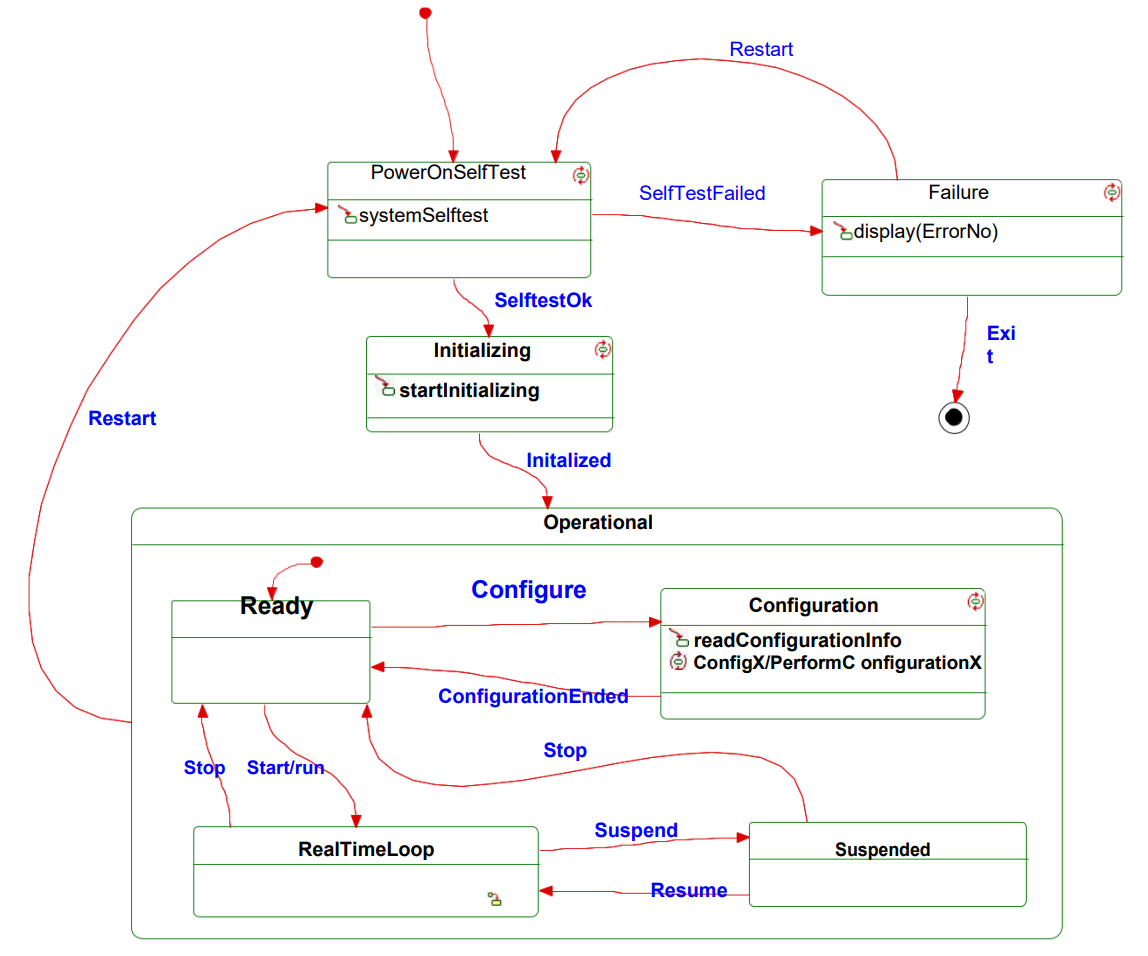
\includegraphics{esx_state_diagram.png}

\subsection{State Pattern}
We used the state pattern to implement the embedded system x within a context class that keeps a reference to the current state.
The context class defines handles for all the events that changes the state of the system. 
For the states we used an abstract class that defines the interface for all the states. Each state is a subclass of this abstract class, and implements the interface.

\subsection{singleton Pattern}
For the state classes, we used the singleton pattern to assure only one instance of each class exists at all times in the system. This simplifies the implementation of the state pattern, 
as we can use the same instance of the state class in the context class. It also reduces the memory usage. 

\subsection{Command Pattern}
The operational state defines some substates, where the transition from the suspended state are implemented using the command pattern. 

\subsection{Active Object Pattern}
The RealTimeLoop state is implemented using the active object pattern. It has three modes which are implemented as singletons substates. 
Each mode can respond to an event, which is handle by the RealTimeLoop state using a queue that handles the events in a FIFO order.

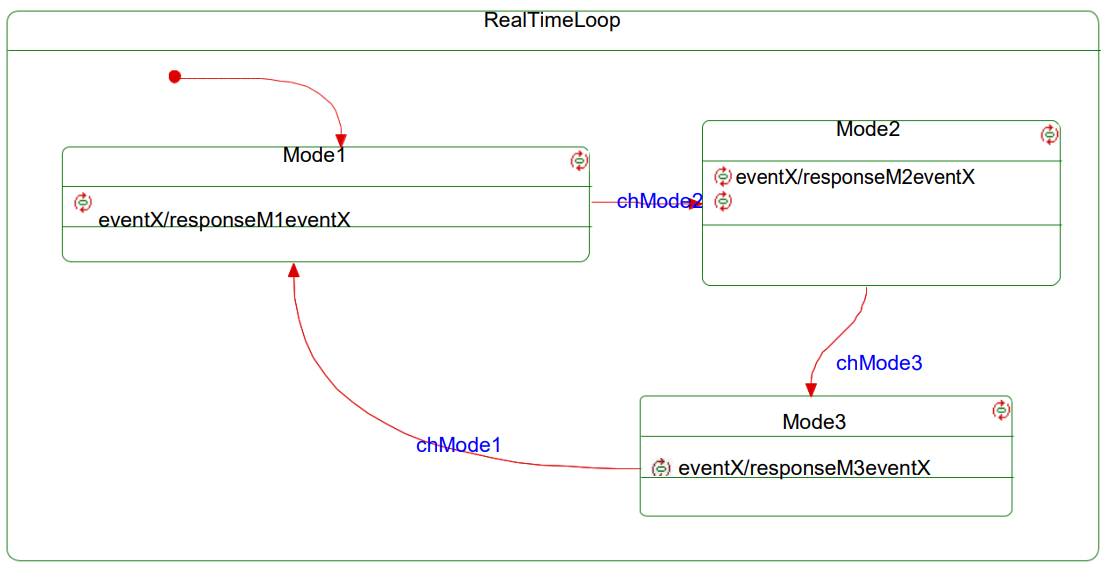
\includegraphics{realtimeloop.png}

\end{document}